\documentclass[preprint,12pt,aps,pra,showkeys,amsmath,amssymb,superscriptaddress,floatfix]{revtex4-2}
\usepackage[T1]{fontenc}
\usepackage[utf8]{inputenc}
\usepackage{amsmath,amssymb,amsthm,mathtools,mathrsfs}
\usepackage{microtype,booktabs,enumitem}
\usepackage{xcolor,tikz,etoolbox}
\usepackage[skins,breakable]{tcolorbox}
\usepackage{needspace}
% Keep diagram geometry independent of REVTeX preprint body spacing.
\AtBeginEnvironment{tikzpicture}{\linespread{1}\selectfont}
\usetikzlibrary{arrows.meta,positioning,calc,fit,decorations.pathreplacing}
\usepackage{graphicx}
\usepackage{hyperref}

\definecolor{MMBlue}{RGB}{0,82,155}
\definecolor{MMOrange}{RGB}{200,80,0}
\tikzset{
 mmnode/.style={draw=MMBlue,rounded corners=2pt,fill=MMBlue!4,align=left,execute at begin node={\raggedright},text width=5cm,font=\fontsize{10}{12}\selectfont,inner sep=6pt},
 mmimport/.style={mmnode,draw=black!65,fill=black!4},
 mmcandidate/.style={mmnode,draw=MMOrange,dashed,fill=MMOrange!5},
 mmrejected/.style={mmnode,draw=black,densely dotted,fill=black!8},
 mmproof/.style={->,thick,MMBlue},
 mmflow/.style={->,semithick,black!70},
 mmrepair/.style={->,dashed,thick,MMOrange},
 mmcandidatearrow/.style={->,dashed,semithick,MMOrange},
 mmnote/.style={font=\scriptsize,fill=white,inner sep=2pt,align=center}}

\usepackage[section]{placeins}
\setlength{\emergencystretch}{3em}
\setlist{itemsep=3pt,topsep=4pt}
\newtheorem{theorem}{Theorem}[section]
\newtheorem{proposition}[theorem]{Proposition}
\newtheorem{lemma}[theorem]{Lemma}
\newtheorem{corollary}[theorem]{Corollary}
\theoremstyle{definition}
\newtheorem{definition}[theorem]{Definition}
\newtheorem{example}[theorem]{Example}
\theoremstyle{remark}
\newtheorem{remark}[theorem]{Remark}
% Avoid isolated statement headings and single-line paragraph fragments.
\BeforeBeginEnvironment{theorem}{\Needspace{6\baselineskip}}
\BeforeBeginEnvironment{definition}{\Needspace{5\baselineskip}}
\BeforeBeginEnvironment{proposition}{\Needspace{5\baselineskip}}
\BeforeBeginEnvironment{lemma}{\Needspace{5\baselineskip}}
\BeforeBeginEnvironment{corollary}{\Needspace{5\baselineskip}}
\clubpenalty=5000
\widowpenalty=5000
\newcommand{\R}{\mathbb R}\newcommand{\Z}{\mathbb Z}\newcommand{\N}{\mathbb N}
\newcommand{\Pa}{\operatorname{Pa}}\newcommand{\Desc}{\operatorname{Desc}}
\newcommand{\cl}{\operatorname{cl}}\newcommand{\cost}{\operatorname{cost}}
\newcommand{\status}{\operatorname{status}}
% Faculty cards: a visual rail groups the five faculties within one agent.
% The rail has no arrowhead and does not represent a proof dependency.
\newcommand{\mmfacultybadge}[1]{%
 \node[circle,draw=MMBlue,line width=1pt,fill=white,
 minimum size=7mm,inner sep=0pt,font=\sffamily\small\bfseries,text=MMBlue]
 at ([xshift=15pt,yshift=-15pt]frame.north west) {#1};}
\newcommand{\mmfacultyrail}{%
 \draw[MMBlue!80,line width=1pt]
 ([xshift=15pt,yshift=2pt]frame.north west)--
 ([xshift=15pt,yshift=-2pt]frame.south west);}
\newtcolorbox{mmfacultybox}[2]{enhanced,breakable,
 colback=MMBlue!4,colframe=MMBlue!4,boxrule=0pt,arc=3pt,
 left=39pt,right=9pt,top=7pt,bottom=7pt,
 before skip=2pt,after skip=2pt,
 fontupper=\normalsize\linespread{1.15}\selectfont,
 overlay unbroken={\mmfacultyrail\mmfacultybadge{#1}},
 overlay first={\mmfacultyrail\mmfacultybadge{#1}},
 overlay middle={\mmfacultyrail},overlay last={\mmfacultyrail}}
\newcommand{\mmfaculty}[3]{%
 \begin{mmfacultybox}{#1}{#2}
 {\sffamily\bfseries\color{MMBlue}#2}\par\smallskip #3
 \end{mmfacultybox}}
\newcommand{\agent}[9]{%
 \Needspace{8\baselineskip}
 \subsubsection{#1}
 \noindent\textbf{Object.} #2\par
 \noindent\textbf{Role.} #3\par\smallskip
 \mmfaculty{E}{Ego}{#4}
 \mmfaculty{M}{Memory}{#5}
 \mmfaculty{I}{Intellect}{#6}
 \mmfaculty{S}{Sense}{#7}
 \mmfaculty{A}{Action}{#8}
 \smallskip\noindent #9\par}

\usepackage{longtable,array}
\providecommand{\tightlist}{\setlength{\itemsep}{2pt}\setlength{\parskip}{0pt}}
% Keep short report abstracts with their title instead of REVTeX's optional preprint break.
\makeatletter
\def\frontmatter@abstract@produce{\par\addvspace{\frontmatter@preabstractspace}%
\begingroup\prep@absbox\unvbox\absbox\post@absbox\endgroup
\addvspace{\frontmatter@postabstractspace}}
\makeatother
\newcommand{\field}[2]{\par\smallskip\noindent\textbf{#1.} #2\par}
\newcommand{\reportcaption}[1]{\par\smallskip{\small\noindent #1\par}}


\hypersetup{colorlinks=true,linkcolor=MMBlue,urlcolor=MMBlue,pdftitle={Fermat's Little Theorem},pdfauthor={Dibakar Sigdel}}

\begin{document}

\title{Fermat's Little Theorem\\[4pt]\large An End-to-End Meta-Math Walkthrough}

\author{Dibakar Sigdel}

\affiliation{Mindverse Computing LLC, Lynnwood, WA 98087, USA}

\date{October 2026}

\begin{abstract}

Multiplication by a nonzero residue permutes a finite set. Comparing its
products gives the desired power, provided the factorial is proved
invertible before cancellation. This report presents a complete proof
relative to explicit imports, a dependency graph, versioned node
contracts, five-faculty activities, exact examples, and an illustrative
repair. The interactions are authored explanations, not a transcript of
deployed agents or a proof-assistant certificate.

\end{abstract}

\maketitle

\linespread{1.12}\selectfont

\noindent\textbf{Project NT-04 \quad Report version 1 \quad Number Theory}

\section{Target and import contract}

\begin{theorem}

For every prime \(p\) and every integer \(a\), \(a^p\equiv a\pmod p\).
Equivalently, for \(p\nmid a\), one has \(a^{p-1}\equiv1\pmod p\).

\end{theorem}

\subsection{Foundations and permitted imports}

\begin{enumerate}
\def\labelenumi{\arabic{enumi}.}
\item
  NT-01/N5, v1: a residue modulo \(m\ge2\) is invertible iff it is
  coprime to \(m\). In particular every nonzero residue modulo a prime
  \(p\) is a unit.
\item
  NT-02/N2, v1: a prime dividing a product divides a factor. An
  injective map from a finite set to itself is bijective; finite
  products in the commutative residue ring are unchanged by permutation.
  No group-order theorem is imported.
\end{enumerate}

\clearpage\section{Node interaction workflow}

\begin{center}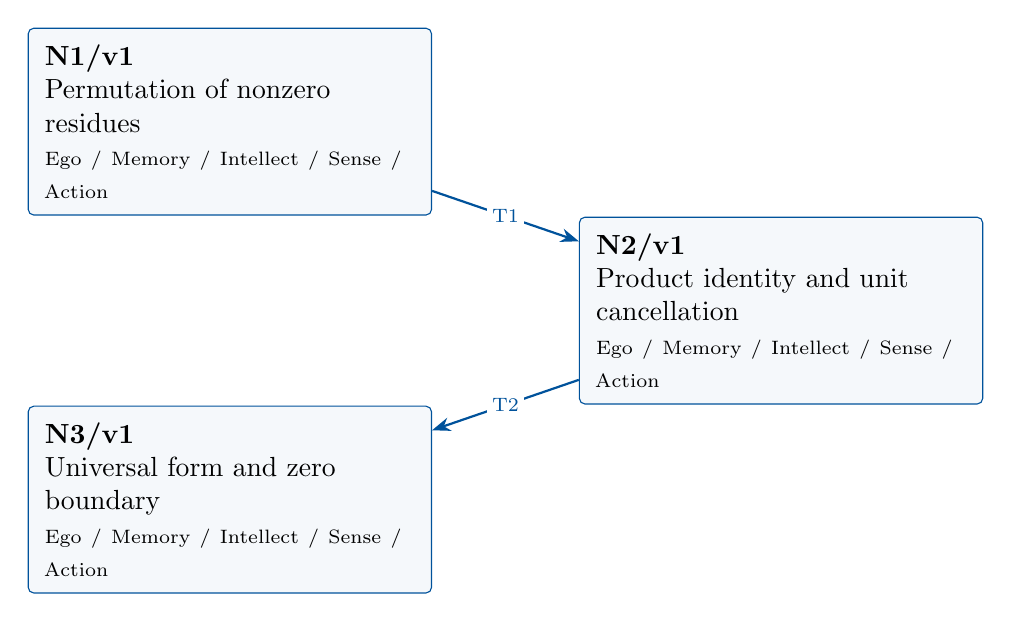
\begin{tikzpicture}[>=Stealth,x=1cm,y=1cm]

\node[mmnode,text width=4.7cm,minimum height=1.35cm] (N1) at (0,0) {\textbf{N1/v1}\\Permutation of nonzero residues\\{\scriptsize Ego / Memory / Intellect / Sense / Action}};

\node[mmnode,text width=4.7cm,minimum height=1.35cm] (N2) at (7,-2.4) {\textbf{N2/v1}\\Product identity and unit cancellation\\{\scriptsize Ego / Memory / Intellect / Sense / Action}};

\node[mmnode,text width=4.7cm,minimum height=1.35cm] (N3) at (0,-4.8) {\textbf{N3/v1}\\Universal form and zero boundary\\{\scriptsize Ego / Memory / Intellect / Sense / Action}};

\draw[mmproof] (N1) to node[mmnote,pos=.5] {T1} (N2);

\draw[mmproof] (N2) to node[mmnote,pos=.5] {T2} (N3);

\end{tikzpicture}\end{center}

\reportcaption{Blue arrows are accepted mathematical dependencies, with exact transfers T1--T2 below. Repair messages are described separately; they are not premises of the proof.}

\subsection{Versioned evidence-transfer ledger}

\begingroup\small\linespread{1.05}\selectfont\renewcommand{\field}[2]{\par\noindent\textbf{#1.} #2\par}

\Needspace{5\baselineskip}\smallskip\noindent\textbf{T1: N1/E1 v1 to N2.1}

\field{Claim}{The map \([j]\mapsto[aj]\) permutes the nonzero classes \(1,\ldots,p-1\)
modulo \(p\).}

\field{Compatibility}{Products run through the same finite set of nonzero classes.}

\field{Evidence}{Node N1 activities below and the continuous proof in Section~\ref{sec:proof}.}

\Needspace{5\baselineskip}\smallskip\noindent\textbf{T2: N2/E2 v1 to N3.1}

\field{Claim}{If \(p\nmid a\), then \(a^{p-1}\equiv1\pmod p\).}

\field{Compatibility}{Apply the power congruence only when \(p
mid a\).}

\field{Evidence}{Node N2 activities below and the continuous proof in Section~\ref{sec:proof}.}

\endgroup

\clearpage\section{Agent roles and five-faculty activities}

\subsection{N1/v1: Permutation of nonzero residues}

\field{Object and role}{Transport a modular multiplication problem into a finite permutation.}

\field{Inputs}{\(p\) prime, \(p\nmid a\); NT-01 inverse criterion and NT-02 Euclid
lemma.}

\mmfaculty{E}{Ego}{Publish a bijection only on the nonzero residue classes.}

\mmfaculty{M}{Memory}{Retain a certified inverse of \(a\) modulo \(p\) and the finite set of
\(p-1\) classes.}

\mmfaculty{I}{Intellect}{Prove the map lands in the set and is injective; finiteness supplies
surjectivity.}

\mmfaculty{S}{Sense}{A nonzero representative modulo a composite need not be a unit.}

\mmfaculty{A}{Action}{If \(p\mid aj\) with \(1\le j<p\), Euclid's lemma would give
\(p\mid j\), a contradiction. Continue with the numbered deductions
below, retaining the exact export.}

\smallskip\noindent\textbf{Numbered mathematical activities}

\begin{enumerate}[label=N1.\arabic*,leftmargin=3.4em]

\item If \(p\mid aj\) with \(1\le j<p\), Euclid's lemma would give
\(p\mid j\), a contradiction.

\item From \(aj\equiv ak\pmod p\), multiply by \(a^{-1}\) to get
\(j\equiv k\pmod p\).

\item The finite self-map is injective and hence a permutation.

\end{enumerate}

\field{Export E1/v1}{The map \([j]\mapsto[aj]\) permutes the nonzero classes \(1,\ldots,p-1\)
modulo \(p\).}

\field{Acceptance gate}{The range contains only nonzero classes and every input has a distinct
image.}

\field{Targeted repair}{If \(p\mid a\), route to the zero case in N3; do not pass a permutation
export to N2.}

\clearpage

\subsection{N2/v1: Product identity and unit cancellation}

\field{Object and role}{Extract the exponent from equal products and justify the cancellation
factor.}

\field{Inputs}{N1/E1; primality of \(p\); NT-01 and NT-02.}

\mmfaculty{E}{Ego}{Publish the power congruence only after certifying the factorial as a
unit.}

\mmfaculty{M}{Memory}{Retain the permutation and the exact product \(P=(p-1)!\).}

\mmfaculty{I}{Intellect}{Compare products before and after multiplication, then multiply by a
certified inverse of \(P\).}

\mmfaculty{S}{Sense}{Do not cancel a merely nonzero integer expression in an arbitrary
residue ring.}

\mmfaculty{A}{Action}{The permutation yields \(a^{p-1}P\equiv P\pmod p\). Continue with the
numbered deductions below, retaining the exact export.}

\smallskip\noindent\textbf{Numbered mathematical activities}

\begin{enumerate}[label=N2.\arabic*,leftmargin=3.4em]

\item The permutation yields \(a^{p-1}P\equiv P\pmod p\).

\item No factor \(1\le j<p\) is divisible by \(p\), so Euclid's lemma gives
\(p\nmid P\).

\item Use the inverse of \(P\) to conclude \(a^{p-1}\equiv1\pmod p\).

\end{enumerate}

\field{Export E2/v1}{If \(p\nmid a\), then \(a^{p-1}\equiv1\pmod p\).}

\field{Acceptance gate}{The equal products and the unit certificate for \(P\) are both present;
\(p=2\) uses \(P=1\).}

\field{Targeted repair}{If the factorial unit claim fails, revisit the prime modulus and
invalidate the cancelled conclusion.}

\clearpage

\subsection{N3/v1: Universal form and zero boundary}

\field{Object and role}{Join zero and nonzero cases and prove the stated equivalence.}

\field{Inputs}{N2/E2 for \(p\nmid a\); arbitrary integer \(a\).}

\mmfaculty{E}{Ego}{Publish the universal claim only after both residue cases are covered.}

\mmfaculty{M}{Memory}{Retain the nonzero-case scope and the inverse of \(a\) only where it
exists.}

\mmfaculty{I}{Intellect}{Multiply by \(a\) in the nonzero case and prove the zero case directly.}

\mmfaculty{S}{Sense}{Do not divide the universal congruence by \(a\) when \(p\mid a\).}

\mmfaculty{A}{Action}{If \(p\nmid a\), multiply N2's congruence by \(a\). Continue with the
numbered deductions below, retaining the exact export.}

\smallskip\noindent\textbf{Numbered mathematical activities}

\begin{enumerate}[label=N3.\arabic*,leftmargin=3.4em]

\item If \(p\nmid a\), multiply N2's congruence by \(a\).

\item If \(p\mid a\), both \(a^p\) and \(a\) are zero modulo \(p\).

\item Conversely for \(p\nmid a\), multiply \(a^p\equiv a\) by \(a^{-1}\).

\end{enumerate}

\field{Export E3/v1}{\(a^p\equiv a\pmod p\) for every integer \(a\), with the equivalent
nonzero formulation.}

\field{Acceptance gate}{Every integer lies in exactly one case and the reverse implication is
restricted to units.}

\field{Targeted repair}{A proposed nonzero formulation for multiples of \(p\) is rejected;
preserve the valid universal form.}

\clearpage\section{Continuous mathematical proof}\label{sec:proof}

\begin{proof}

Assume first \(p\nmid a\). The map \([j]\mapsto[aj]\) on the nonzero
residue classes modulo \(p\) is well-defined and has nonzero values: if
\(p\mid aj\), Euclid's lemma and \(p\nmid a\) would force \(p\mid j\).
Moreover, \(a\) has an inverse by NT-01, so \(aj\equiv ak\) implies
\(j\equiv k\). This is an injective self-map of a finite set, hence a
permutation (N1).

Multiplying all its values and comparing with the original product gives
(N2) \[a^{p-1}(p-1)!\equiv(p-1)!\pmod p.\] Each factor \(1,\ldots,p-1\)
is not divisible by \(p\). Repeated Euclid's lemma implies
\(p\nmid(p-1)!\), so its gcd with \(p\) is \(1\). The inverse criterion
therefore justifies multiplying by the inverse of the factorial. This
yields \(a^{p-1}\equiv1\pmod p\). For \(p=2\), the product is simply
\(1\), so the same argument applies.

Multiplying the nonzero-case congruence by \(a\) yields \(a^p\equiv a\).
If \(p\mid a\), both sides are zero modulo \(p\), proving the universal
formulation (N3). Conversely, for \(p\nmid a\), multiply the universal
formulation by the inverse of \(a\) to recover \(a^{p-1}\equiv1\).
Residue classes cover negative as well as nonnegative integers.

\end{proof}

\section{Worked orchestration}

For \(a=3,p=7\), N1 constructs the permutation
\[1,2,3,4,5,6\ \longmapsto\ 3,6,2,5,1,4\pmod7.\] N2 uses
\(6!=720\equiv6\pmod7\), whose inverse is \(6\), to cancel the product.
Thus \(3^6=729=104\cdot7+1\). Multiplying by \(3\) gives
\(3^7\equiv3\pmod7\). For \(a=14\), N3 instead uses the zero case
\(14^7\equiv14\equiv0\pmod7\); it does not assert \(14^6\equiv1\).

\subsection{Boundary and hypothesis audit}

\begin{itemize}
\item
  At \(p=2\), odd \(a\) satisfies \(a\equiv1\pmod2\), while even \(a\)
  uses the zero case.
\item
  Primality cannot simply be dropped: \(2^4\equiv0\not\equiv2\pmod4\).
  Even coprimality alone does not preserve the exponent \(m-1\):
  \(3^3\equiv3\not\equiv1\pmod4\).
\item
  Modular cancellation can fail: \(2\cdot1\equiv2\cdot4\pmod6\), but
  \(1\not\equiv4\pmod6\).
\end{itemize}

\section{Illustrative failure and repair}

This is a deliberately authored teaching trace. A diagnostic asks for
correction; it cannot prove a predecessor by importing its descendant's
conclusion. A revised export must be checked before its consumers are
reused.

\field{Candidate}{N2 cancels a factorial modulo an arbitrary positive modulus merely
because the factorial is a nonzero integer.}

\field{Detection}{Sense supplies \(2\cdot1\equiv2\cdot4\pmod6\); the common factor \(2\)
is not a unit.}

\field{Correction}{Memory retrieves the inverse criterion. Under the actual prime-modulus
contract, Action proves \(p\nmid(p-1)!\) before cancellation.}

\field{Recheck}{Recompute N2's product deduction and N3's nonzero branch; the zero
branch remains a separate direct argument.}

\field{Publication}{Ego exports Fermat's theorem for prime moduli. A composite-modulus
result would require a different exponent and proof.}

\section{Reusable result and provenance}
Reusable exports retain each node's version 1 statement, assumptions, and proof.
The final export is the theorem in Section 1, proved relative to its declared imports.

\smallskip\noindent\textbf{Source record.} Adapted from the original project Markdown:
\par\noindent\nolinkurl{fermat-s-little-theorem.md}\par
Typography, workflow conventions, and faculty cards follow the workspace Meta-Math
manuscript. This authored exposition does not claim formal certification.
\end{document}
